\section{Metodologia}

\subsection{Delineamento e linhas de avaliação}

O estudo é uma comparação de políticas de despacho em simulação de eventos discretos \cite{banks2010}, com os mesmos pedidos, frota, jornadas, compromissos, método de distância e parâmetros em todas as políticas. Há duas linhas de avaliação, relatadas separadamente e nunca somadas: a linha \textbf{A}, \enquote{avaliação contrafactual por simulação com entradas históricas}, e a linha \textbf{B}, \enquote{avaliação em cenários sintéticos}. Em ambas, o que se mede é a diferença entre políticas \emph{dentro do simulador}. A política de referência é um simulador do despacho pelo veículo mais próximo; não é a operação manual real, que não foi observada nem reproduzida, e a comparação só permite afirmar o que o simulador mostra sobre a mudança de política.

\begin{table}[!htb]
\caption{Políticas comparadas}\label{tab:politicas}
\centering\fontetabela
\begin{tabular}{@{}>{\raggedright\arraybackslash}p{13mm}>{\raggedright\arraybackslash}p{32mm}>{\raggedright\arraybackslash}p{52mm}>{\raggedright\arraybackslash}p{46mm}@{}}
\toprule
Código & Política & Instante de decisão & Regra de escolha \\
\midrule
A & mais próximo, imediato & na chegada do pedido (fila por ordem de chegada se não houver veículo elegível) & veículo elegível mais próximo \\
B & mais próximo, em lotes & lotes a cada 60 s; pedidos ordenados por chegada e, em empate, por identificador & cada pedido recebe o veículo elegível mais próximo ainda livre \\
C & atribuição conjunta (Húngaro), em lotes & lotes a cada 60 s & solução lexicográfica da equação~\ref{eq:obj} \\
\bottomrule
\end{tabular}
\fonte{elaborada pelos autores a partir da implementação (\texttt{B0\_imediato\_atual}, \texttt{B\_lote60s\_guloso\_fifo}, \texttt{B\_lote60s\_hungaro}).}
\end{table}

O contraste principal é C×A (mudança integral de política, fixado antes das execuções). C×B isola a atribuição conjunta do efeito do lote (mesma janela de 60 s), e B×A mostra o efeito do lote com a regra sequencial. A ordem de B (chegada e depois identificador) é a mesma do despacho imediato e foi definida antes de qualquer resultado, sem depender de C.

\subsection{Implementação do despacho em lotes}

Os lotes ocorrem em instantes múltiplos de 60 s contados da meia-noite. Um pedido recebido espera o próximo instante de lote; sua espera é contada desde a chegada. Um veículo que termina uma corrida só volta a ser candidato no lote seguinte. A cada instante, o simulador monta, para cada pedido pendente, a lista de veículos elegíveis ordenada por distância, chama a política e valida o resultado: o simulador aborta se um par for inelegível ou duplicado. Pedidos não atendidos voltam ao conjunto pendente e expiram após a paciência. O Algoritmo~\ref{alg:lote} e a Figura~\ref{fig:fluxo} resumem o procedimento.

\begin{algoritmo}[!htb]
\caption{Despacho em lotes de 60 s (políticas B e C)}\label{alg:lote}
\fontetabela
\begin{tabular}{@{}l@{}}
\textbf{para cada} instante de lote $t$ \textbf{faça} \\
\quad $P \leftarrow$ pedidos pendentes com chegada $\le t$, ordenados por (chegada, identificador) \\
\quad \textbf{para cada} $r\in P$: $L_r \leftarrow$ veículos elegíveis em $t$, por distância crescente \\
\quad \textbf{se} B: \textbf{para} $r\in P$ \textbf{em ordem}: atribuir o primeiro $v\in L_r$ ainda livre \\
\quad \textbf{se} C: montar a matriz ampliada (eq.~\ref{eq:obj}) e resolver pelo Húngaro \\
\quad validar pares (únicos e elegíveis); para cada par, ocupar $v$ e atualizar posição e liberação \\
\quad pedidos sem par permanecem pendentes até $t+60$ s ou até esgotar a paciência \\
\end{tabular}
\fonte{elaborado pelos autores a partir de \texttt{simulation/engine.py} e \texttt{assignment/dispatch.py} (no código congelado, \texttt{v2/sim.py} e \texttt{comparacao/despacho.py}).}
\end{algoritmo}

\begin{figure}[!htb]
\caption{Fluxo da atribuição em lote}\label{fig:fluxo}
\centering
\begin{tikzpicture}[node distance=7mm, box/.style={draw, rounded corners=2pt, align=center, font=\fontsize{9}{10}\selectfont, minimum height=10mm, text width=34mm}, >=Stealth]
\node[box](a){Instante de lote $t$ (múltiplo de 60 s)};
\node[box,right=of a](b){Pedidos pendentes (chegada $\le t$)};
\node[box,right=of b](c){Veículos elegíveis (livres, no raio, sem conflito)};
\node[box,below=of c](d){Matriz de custos $c_{rv}$ (km)};
\node[box,left=of d](e){Escolha: B (mais próximo) ou C (Húngaro)};
\node[box,left=of e](f){Validação: pares únicos e elegíveis};
\node[box,below=of f](g){Atualização de ocupação, posição e liberação};
\node[box,right=of g](h){Pedidos sem par seguem para $t+60$ s};
\draw[->](a)--(b);\draw[->](b)--(c);\draw[->](c)--(d);\draw[->](d)--(e);\draw[->](e)--(f);\draw[->](f)--(g);\draw[->](g)--(h);
\end{tikzpicture}
\par\fonte{elaborada pelos autores a partir do simulador (\texttt{simulation/engine.py}; no código congelado, \texttt{v2/sim.py}).}
\end{figure}

\subsection{Linha A: dados históricos da operação V1 Viagens}

Os dados vêm de uma operação de transporte por aplicativo na Grande Vitória (ES), delimitada como produto V1, região 1 (Grande Vitória), serviços 1, 11, 12 e 19, excluídos os serviços Prime. As entidades usadas, extraídas em modo somente leitura do banco operacional (SQL Server) e do índice de posições de ofertas (Elasticsearch), são: solicitações (origem, destino, instante de registro, tipo), jornadas de motoristas, compromissos externos, vínculos entre veículo e condutor, posições dos veículos ofertados (instantâneos a cada cerca de 2 minutos) e cadastro de veículos, uma fotografia única extraída em 08/11/2026. A telemetria de terceiros existe só em fevereiro e março e \textbf{não} é usada: nenhuma quilometragem do estudo é odométrica ou validada por ela. Os arquivos derivados são armazenados em Parquet com manifesto e SHA-256 por dia; a extração depende de consultas somente leitura e não de plataformas em nuvem.

A Tabela~\ref{tab:periodos} traz os períodos e os volumes. O treino e a validação foram usados no desenvolvimento e na escolha da política; a replicação e a avaliação final nunca haviam sido simuladas antes da execução congelada.

\begin{table}[!htb]
\caption{Períodos e volumes da linha A (pedidos de tempo real, sem agendados)}\label{tab:periodos}
\centering\fontetabela
\begin{tabular}{@{}llrrrr@{}}
\toprule
Período & Datas (2026) & Dias & Pedidos & Motoristas/dia (média) & Compromissos \\
\midrule
Treino & 01/02--15/03 & 43 & 51.909 & 106,8 & 1.458 \\
Validação & 16/03--31/03 & 16 & 20.178 & 111,3 & 675 \\
Replicação & 16/09--30/09 & 15 & 16.918 & 86,7 & 674 \\
Final & 01/10--25/10 & 25 & 23.523 & 74,3 & 842 \\
\bottomrule
\end{tabular}
\fonte{\texttt{reports/atribuicao\_final/volumes\_por\_periodo.json}. Pedidos agendados ficam fora; pedidos cancelados permanecem como demanda.}
\end{table}

Regras de construção, todas fixadas antes da execução congelada:
\begin{alineas}
\item \textit{Elegibilidade do dia}: entidades do dia presentes, ao menos 300 instantes de posição e ao menos 200 pedidos; os 15 dias de setembro e os 25 de outubro cumpriram (mínimos de 702 instantes e 459 pedidos), sem exclusão.
\item \textit{Disponibilidade}: a presença de um veículo no registro de ofertas não prova disponibilidade, pois esse registro inclui veículos ocupados e subcobre parte da atividade. A janela de um motorista (cenário J) é a jornada registrada interseccionada com a presença no registro, estendida por lacunas de até 1.200 s; lacunas maiores ficam como desconhecidas e fora da janela; compromissos externos bloqueiam o motorista. A jornada usada é a realizada, informação disponível só retrospectivamente ao avaliador, comum a todas as políticas.
\item \textit{Posição inicial}: primeira posição observada do motorista na janela. Depois disso, ocupação e posição vêm das corridas que o próprio simulador atribui; as corridas históricas não entram como compromissos.
\item \textit{Parâmetros}: raio de despacho de 4,5 km em linha reta, velocidade de 16,079 km/h, fator rua/reta de 1,3012 e paciência de 180 s, herdados da calibração com dados de março e não recalibrados para setembro e outubro.
\item \textit{Tentativas}: novas solicitações do mesmo passageiro em pouco tempo não foram deduplicadas, e cancelamentos posteriores à atribuição não são modelados.
\item \textit{Privacidade}: identificadores de motoristas, veículos e passageiros são pseudonimizados por HMAC-SHA256 com segredo fora do repositório; só agregados são reportados, em conformidade com a \citeonline{brasil2018}.
\end{alineas}

O que a política conhece em cada lote é só o que já aconteceu: pedidos chegados e veículos elegíveis no instante. O ambiente retrospectivo (jornadas realizadas e compromissos) é construído com dados completos do dia e é igual nas três políticas.

Para separar o que a política pode saber do que só o avaliador sabe, a Tabela~\ref{tab:info} distingue três planos de informação.

\begin{table}[!htb]
\caption{Planos de informação na linha A}\label{tab:info}
\centering\fontetabela
\begin{tabular}{@{}p{34mm}p{62mm}p{52mm}@{}}
\toprule
Plano & Conteúdo & Disponível à política? \\
\midrule
Política (instante $t$) & pedidos chegados até $t$; veículos online, livres e elegíveis em $t$; distâncias estimadas & sim \\
Ambiente retrospectivo & janelas de jornada realizadas, presença no registro de ofertas, compromissos externos, cadastro de veículos & não: reconstruídos com o dia completo; iguais nas três políticas \\
Hipóteses de simulação & raio, velocidade, fator rua/reta, paciência, posição inicial, cenário J, ausência de aceite e de cancelamento pós-atribuição & não: parâmetros fixos, herdados de março \\
\bottomrule
\end{tabular}
\fonte{elaborada pelos autores a partir da documentação do experimento.}
\end{table} O km é estimado (distância em linha reta vezes 1,3012), não medido por odômetro.

\subsection{Linha B: cenários sintéticos}

O recorte geográfico reúne os municípios de Vitória, Vila Velha, Serra e Cariacica, com malhas do IBGE \cite{ibgemalhas}, e a rede viária do OpenStreetMap \cite{osm}, obtidas em 08/11/2026 e registradas com SHA-256. O instantâneo do OpenStreetMap é o da consulta à API Overpass (versão 0.7.62.11) de 08/11/2026, às 15:13 UTC, com 36.350 elementos de via, licença ODbL; a malha do IBGE usa o sistema WGS84 (EPSG:4326). A Figura~\ref{fig:mapa} mostra o recorte. Pontos de parada são nós viários, um por célula H3 de resolução 8 \cite{uberh3}, a no máximo 20 km por via, ida e volta, do centro de Vitória; as distâncias são caminhos mínimos pela rede (Dijkstra). As células H3 servem só para escolher os pontos de parada e definir as zonas do gerador de demanda (e para o mapa); não participam da atribuição, que depende apenas das distâncias por via. Em resumo, a rede viária vem do OpenStreetMap e dá o modelo de custo dos deslocamentos; o mapa da Figura~\ref{fig:mapa} é de apresentação. A geografia é real; a demanda, a frota, as jornadas e as velocidades são hipóteses experimentais do gerador (versão 1.0.0), com parâmetros registrados. A frota tem 100 veículos, com jornadas de 9 horas iniciadas às 6, 8, 10 ou 12 h, velocidade de 25 km/h, raio de despacho de 8 km por via e paciência de 600 s. Os cenários principais são S1 (demanda uniforme), S2 (concentrada), S3 (frota inicialmente desequilibrada), S4 (mudança inesperada da demanda) e S5 (demanda que migra de região); 17 variantes alteram a relação frota/demanda (4, 8 ou 14 pedidos por veículo) ou parâmetros de previsão, que não afetam o despacho (22 cenários no total). As concentrações de demanda são hipóteses e não representam padrões reais.

\begin{figure}[!htb]
\caption{Recorte geográfico da linha B: células H3 de resolução 7 com pontos de parada}\label{fig:mapa}
\centering
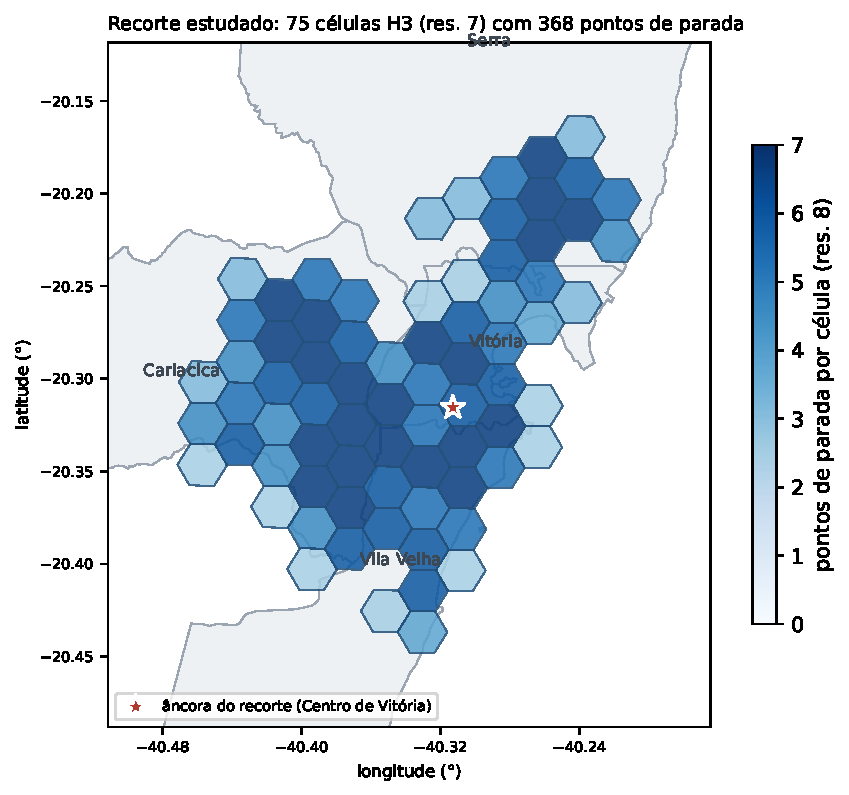
\includegraphics[width=0.78\linewidth]{figures/mapa_recorte_h3.pdf}
\par\fonte{elaborada pelos autores com limites municipais do IBGE e vias do OpenStreetMap (ODbL); a cor indica o número de pontos de parada de resolução 8 por célula; a estrela marca o ponto de referência do recorte, no centro de Vitória. Mapa ilustrativo: não mostra demanda, veículos nem rotas.}
\end{figure}

A Figura~\ref{fig:mapa} mostra que o recorte (75 células e 368 pontos de parada) cobre a ilha de Vitória e partes de Vila Velha, Cariacica e Serra, e não toda a região metropolitana; é um recorte experimental, não um limite administrativo nem a área de atuação de uma empresa. Sobre a rede: o arquivo do OpenStreetMap contém 521 trechos marcados como ponte ou viaduto, entre eles a Ponte Deputado Darcy Castello de Mendonça, a Ponte Governador Gerson Camata, a Ponte do Príncipe e a Ponte Florentino Avidos. As verificações feitas foram estruturais: o grafo do recorte é conexo (as distâncias entre os 368 pontos são todas finitas), a distância por via nunca é menor que a distância em linha reta, e a razão entre as duas, em mediana, é de 1,45 entre Vitória e Vila Velha e de 1,34 dentro de Vila Velha, de modo que há travessia mapeada entre a ilha e o continente. \textbf{Não} se verificou ponte a ponte se cada ligação existente está mapeada nem se validaram tempos de percurso contra medições; não se afirma, portanto, que as pontes estejam corretamente representadas, e congestionamento e travessias bloqueadas não são modelados.

Cada cenário foi simulado com 40 sementes (20001--20040), reservadas antes da execução. A unidade de análise é a semente. As sementes de desenvolvimento (101--120) foram usadas antes, e os resultados das 40 sementes finais foram vistos antes de os autores decidirem adotar o método. Por isso, a linha B é tratada como evidência \textbf{exploratória e complementar}: os 22 cenários compartilham rede, frota e geração de pedidos (não são 22 confirmações independentes), e as sementes finais foram examinadas antes da adoção; ela ilustra o comportamento do método em condições controladas e não substitui a linha A.

\subsection{Desenho, congelamento e origem da janela de 60 s}

A janela de 60 s foi escolhida no treino real (01/02--15/03) entre 30 s e 60 s, por regra fixada em plano escrito antes da primeira execução: entre as políticas com serviço preservado e limite superior do IC95\% abaixo de zero, a de menor km, desempatando por simplicidade e tempo. A validação (16--31/03) e a avaliação sintética final foram vistas antes da decisão de adotar o método, embora não tenham escolhido a janela nem o algoritmo. Em 09/11/2026, antes de simular setembro e outubro, congelou-se o código (SHA-256 de 151 arquivos), os parâmetros, as políticas, os contrastes e os critérios, e o executor se recusa a rodar se o código mudar. Setembro foi executado antes de outubro, uma vez, sem ajuste entre eles, com 0 falhas técnicas e 0 reexecuções. O Apêndice~\ref{ap:repro} reúne os hashes e as verificações. Por isso, setembro e outubro são evidência fora do período de seleção, mas não totalmente independente: mesma empresa, região, simulador e parâmetros calibrados em março. Cada período é uma observação, não 40 experimentos independentes.

\subsection{Métricas e estatística}

Para a política $\pi$ em um período, o km vazio é a soma das distâncias de aproximação dos pares despachados, $K_\pi=\sum_{(r,v)\in D_\pi} c_{rv}$, com $c_{rv}=1{,}3012\,h_{rv}$ e $h_{rv}$ a distância em linha reta (km) na linha A e a distância por via na linha B; esta linha não tem reposicionamento nem retorno. As diferenças são
\begin{equation}
\Delta K = K_C - K_{ref}, \qquad \Delta\% = 100\,\frac{K_C-K_{ref}}{K_{ref}}, \label{eq:delta}
\end{equation}
em km e em \%, onde \textbf{valor negativo significa redução}. O atendimento é $N_\pi/N$, com $N_\pi$ os pedidos atendidos e $N$ os pedidos elegíveis (igual em todas as políticas); reporta-se $\Delta N=N_C-N_{ref}$ e a diferença em pontos percentuais, $100\,\Delta N/N$, que tem como denominador o universo elegível; a variação relativa aos atendidos da referência, $100\,\Delta N/N_{ref}$, é outra quantidade e é identificada como tal quando citada. A espera de um pedido atendido é o tempo entre a chegada e o despacho mais o deslocamento estimado até a origem, e inclui, portanto, o atraso até o fechamento do lote. \textbf{A espera é calculada apenas entre os pedidos atendidos de cada política} (média e P90, nas tabelas e no texto). Como os conjuntos de atendidos diferem entre políticas, a comparação de espera é descritiva e sujeita a seleção: uma política que atende pedidos que a outra deixa expirar pode ter espera média maior ou menor por esse motivo, e a espera não é, por si só, evidência de melhora do serviço.

Critérios de preservação do atendimento (fixados antes, sem acordo de nível de serviço com a empresa): \textbf{E1}, nenhuma violação de compromisso causada pela política; \textbf{E2}, $N_C\ge N_{ref}$ no período; \textbf{E3}, P90 da espera agregada de C não superior ao da referência. A classe \texttt{redução com serviço preservado} exige limite superior do IC95\% abaixo de zero e E1--E3.

A unidade de análise é o dia. Para cada dia $d$, calcula-se $\delta_d=K_{C,d}-K_{ref,d}$ (comparação pareada) e o IC95\% da média de $\delta_d$ por \textit{bootstrap} de blocos móveis de 7 dias (10.000 reamostragens, semente 20261108), que respeita a dependência temporal entre dias. Na linha B, a unidade é a semente. Um intervalo que inclui zero indica que a diferença não é distinguível de zero com os dados, e não que as políticas sejam equivalentes. Na linha B, os testes confirmatórios (5 cenários principais $\times$ 4 variantes de despacho em lote avaliadas no experimento, contra A: 20 testes) usam correção de Holm, e os demais cenários são exploratórios. Totais por período e diferença média diária são ambos reportados; os totais respondem pela soma de km, e os intervalos, pela variação entre dias.
